% =====================================================================
% CGA-Agent (English, LaTeX route) -- regenerated through the JiuwenSwarm
% paper pipeline. Reference: paper/paper.docx (imported CGA-Agent paper).
% Output is a NEW file; the original paper.docx / paper.pdf are untouched.
% Compile: xelatex -interaction=nonstopmode -halt-on-error paper_v5_en.tex (twice)
% =====================================================================
\documentclass[journal,10pt,a4paper]{IEEEtran}
\usepackage{amsmath,amssymb}
\usepackage{graphicx}
\usepackage{booktabs}
\usepackage{array}
\usepackage{tikz}
\usetikzlibrary{arrows.meta,positioning,fit,backgrounds,shapes.geometric,calc}
\usepackage{pgfplots}
\pgfplotsset{compat=1.17}
\usepackage{xcolor}
\usepackage[hidelinks]{hyperref}

\hyphenation{op-tical net-works semi-conduc-tor}

% --- layout tuning to reach the 15-page target ---
\setlength{\abovecaptionskip}{1pt}
\setlength{\belowcaptionskip}{0pt}
\setlength{\textfloatsep}{4pt plus 1pt minus 1pt}
\setlength{\floatsep}{4pt plus 1pt minus 1pt}
\setlength{\intextsep}{4pt plus 1pt minus 1pt}
\setlength{\abovedisplayskip}{3pt plus 1pt minus 1pt}
\setlength{\belowdisplayskip}{3pt plus 1pt minus 1pt}
\setlength{\jot}{2pt}
\linespread{0.96}

\begin{document}

\title{CGA-Agent: Structured Context Engineering and Claim-Evidence Guardrails for Trustworthy Multi-Agent LLM Systems}

\author{Author Name1, Author Name2, Author Name3\\
\textit{1 School of Computer Science and Technology, University;}\\
\textit{2 Corresponding author. E-mail: author@example.edu.cn}}

\maketitle

\begin{abstract}
Large language model (LLM) based agents have become a pivotal paradigm bridging language understanding and real-world action, yet they exhibit three structural deficiencies on long-horizon tasks: contexts are concatenated as untyped text so that critical constraints are diluted; generated conclusions carry no verifiable evidence anchor so that hallucinations propagate along the reasoning chain; and multi-agent collaboration degenerates into unconstrained aggregation of opinions. This paper proposes CGA-Agent (Context-Guardrail Agent), a layered multi-agent framework founded on structured context engineering and evidence guardrails. We contribute four mechanisms. First, a structured context engineering paradigm that decomposes the context into four typed slots --- task-specification, evidence, reasoning-trace and long-term-memory --- together with an optimization model that allocates a fixed context budget across slots so that high-information-density content is retained. Second, a Claim-Evidence guardrail that segments generated text into minimal verifiable units termed claims, binds each claim to retrieved evidence, and enforces a triple gate of coverage, entailment and traceability; claims failing the gate are intercepted and trigger targeted rewriting, rendering hallucinations localizable, interceptable and auditable. Third, a memory write-gate that scores candidate memories by a joint criterion of information gain, temporal decay, usage frequency and redundancy, suppressing memory pollution at the source. Fourth, uncertainty-driven adaptive planning and claim-level consistency arbitration, so that the agent expands search depth under epistemic uncertainty, contracts its budget otherwise, and aggregates collaborators by evidence strength rather than by expressed confidence. Experiments on HotpotQA, StrategyQA, ToolBench and a self-constructed evidence-annotated benchmark CE-Bench, using three random seeds and six baselines, show that CGA-Agent attains an average task success rate of 77.9\%, exceeding the strongest baseline AutoGen by 9.4 points and vanilla prompting by 32.9 points. Evidence coverage rises from 76.1\% to 91.7\%, the unsupported-claim rate drops from 17.8\% to 6.4\%, and the mis-citation rate reaches 3.1\%. The average token cost is 7.15K, lower than AutoGen's 13.2K, constituting a Pareto improvement on the cost-performance plane. Ablation identifies the evidence guardrail and structured context as the two most critical modules, contributing 11.6 and 9.0 points respectively. Under 50\% distractor injection CGA-Agent retains 59.1\% success rate with roughly 7 points less degradation than baselines. We further delimit applicability boundaries, failure modes and deployment paths in scientific assistance, enterprise knowledge engineering and industrial operations.
\end{abstract}

\begin{IEEEkeywords}
large language models, autonomous agents, context engineering, evidence guardrails, multi-agent collaboration, adaptive planning, trustworthy artificial intelligence
\end{IEEEkeywords}

% =====================================================================
\section{Introduction}
\subsection{Background and Motivation}
Since 2020, Transformer-based large language models (LLMs) have advanced along three axes --- parameter scale, training corpora and alignment techniques --- acquiring for the first time a general capability to follow open-domain instructions, perform multi-step reasoning and emit structured output. An LLM alone, however, is a closed mapping function: it consumes text and emits text, neither acquiring external information nor altering the state of its environment. This limitation motivated the agent paradigm, which couples an LLM as reasoning kernel with tools, memory and environmental feedback, moving the model from answering questions to completing tasks.

When an agent can autonomously decompose goals, invoke retrieval and computation tools, and correct itself after failure, its applicability extends from text generation to hypothesis testing, software engineering automation, enterprise process orchestration and industrial maintenance. Open-source frameworks such as ReAct, Reflexion and AutoGen were widely integrated within two years, and an engineering ecosystem of tool protocols, orchestration engines and observability facilities has emerged. Agent reliability therefore directly determines whether LLMs can enter mission-critical business that tolerates no error.

Capability expansion and reliability degradation have nevertheless occurred in lockstep. Existing agents remain markedly fragile on long-horizon, multi-hop and strongly constrained tasks: an error early in the reasoning chain is not detected downstream and propagates; retrieved evidence is not explicitly bound to the final conclusion, so that grounded conclusions and plausible hallucinations are superficially indistinguishable; and in multi-agent settings roles tend to concur rather than falsify one another, so that collaboration gains decay rapidly as task complexity grows. In medicine, law, finance and industrial control such fragility is the primary obstacle to deployment. Making agent conclusions verifiable, traceable and auditable without materially increasing inference cost is therefore an urgent problem.

We condense the resulting research gaps into four actionable defects that motivate our design. \textbf{Defect 1: context mismatch and constraint dilution.} Agents typically concatenate system instructions, task description, retrieved evidence, execution traces and memory entries into a single untyped sequence. Critical constraints such as output format, prohibited behaviours and freshness requirements are thereby submerged by low-density content, and compliance degrades as the context grows; moreover the model cannot distinguish a binding specification from an merely indicative retrieval result, leading to confusion between constraints and evidence. \textbf{Defect 2: undetectable hallucination propagation.} Error detection is usually applied to the final answer, whereas in long-horizon tasks errors arise in intermediate steps: one faulty entity resolution or one failed tool call places all subsequent reasoning on a false premise. Since intermediate conclusions are not required to bind evidence, such errors remain invisible during generation and surface only when the final answer is judged wrong --- too late to trace the offending step, let alone to produce an auditable record of which claim lacked support. \textbf{Defect 3: memory pollution and collaboration degeneration.} Long-term writes lack quality gating, so duplicate entries, stale conclusions and unverified inferences are persisted and then repeatedly retrieved and amplified. In multi-agent settings the absence of arbitration grounded in evidence strength makes roles mutually confirmatory, and collaboration gains fall below single-agent performance on complex tasks. \textbf{Defect 4: the rigid trade-off between cost and accuracy.} The direct route to reliability is more inference budget --- more samples, more reflection rounds, more tool calls --- but cost grows near-linearly with reliability, rendering the combination of high reliability and low cost unreachable under current frameworks. The absence of on-demand budget allocation is the direct cause of agents being affordable yet ineffective in high-value settings.

\subsection{Related Work}
\subsubsection{Single-agent research: from symbolic reasoning to reinforcement learning}
Early agent research was dominated by symbolism: the BDI (Belief-Desire-Intention) model characterised behaviour as a reasoning relation among beliefs, desires and intentions, while the POMDP framework placed environmental uncertainty, observation sparsity and action selection in one probabilistic model, making action under incomplete information computable. This stage established the formal boundaries of the agent but depended heavily on hand-crafted knowledge and rules, limiting generalisation to open-domain tasks. A second stage, driven by deep reinforcement learning, let agents acquire policies from high-dimensional observations through interaction, surpassing human level on Atari, Go and robotic control. Its capacity remained bound to a specific environment and reward function, however: learned policies transfer poorly to new task descriptions, and sample efficiency is low while reward design is costly. Agents thus remained task-specific, lacking a general language interface.

\subsubsection{Multi-agent systems: cooperation, games and emergence}
Multi-agent systems study the coordination of autonomous agents in a shared environment. Early results addressed task allocation and resource competition through distributed constraint optimisation, contract-net protocols and auction mechanisms; with deep learning, MADDPG and QMIX handled non-stationarity via centralised training with decentralised execution and demonstrated learnable cooperative strategies in complex adversarial environments. The central insight is that collective performance is not the sum of individual performance and that protocol design often matters more than individual capability. Negative failure modes have been repeatedly observed, including social loafing through diffusion of responsibility and group polarisation: when individuals weight others' expressed opinions above their own evidence, small initial biases are amplified each round until the group converges on a false consensus. These findings carry direct warnings for LLM-based multi-agent systems, which precisely lack mechanisms that suppress concurrence.

\subsubsection{LLM agents: tools, memory and planning}
LLMs gave agents a general language interface and shifted the focus to three pillars. In reasoning and planning, chain-of-thought (CoT) prompting improved multi-step accuracy by generating explicit intermediate steps; Least-to-Most and Tree-of-Thoughts organised reasoning as decomposition sequences and tree search, trading additional inference budget for correctness on hard problems. In action and tool use, ReAct alternated reasoning with acting so that the model selects a tool conditioned on the current observation, while Toolformer learned in a self-supervised manner when to insert API calls. In memory and reflection, Reflexion introduced verbal self-feedback that stores failure experience in natural language and reuses it on later attempts, and Generative Agents and MemGPT explored memory-stream retrieval and operating-system-style hierarchical memory respectively.

Multi-agent work progressed in parallel: AutoGen abstracts multi-agent sessions as programmable conversation graphs, MetaGPT constrains role division through standard operating procedures with intermediate artefact validation, and CAMEL studies autonomous collaboration under role playing. Multi-agent debate, in which several instances interrogate one another, improves factuality and outperforms self-consistency sampling on some reasoning benchmarks. Retrieval-augmented generation mitigates factual hallucination by introducing external retrieval, and Self-RAG and CRAG further let the model decide when to retrieve and critically filter retrieved results.

\subsubsection{Critical assessment}
Taken together, existing work has advanced capability construction substantially but leaves clear gaps in reliability assurance. First, planning, memory, tool use and collaboration have mostly been proposed as independent contributions, without joint optimisation or mutual constraint inside one framework; the interface between modules is typically free text, so constraints are diluted in transit. Second, factuality improvements rely mainly on indirect proxy signals, such as repeated sampling with voting or self-critique, which cannot yield an explicit conclusion-to-evidence correspondence and therefore cannot support post-hoc audit. Third, multi-agent aggregation is usually confidence voting, yet expressed confidence in LLMs is systematically biased with respect to true accuracy, so highly confident but erroneous claims tend to dominate. Fourth, evaluation lacks a unified trustworthiness-oriented metric system: incompatible settings make reported accuracies non-comparable. The architecture taxonomy in Table~\ref{tab:taxonomy} summarises how existing designs differ along the control dimension.

\subsubsection{Verification-centric, budget-aware and modular-context baselines}
Several recent lines are adjacent to our design. Claim- and entity-level verification is pursued by Chain-of-Verification [23] and by recent verifiers such as MedRAGChecker [35] and EAEV [36]; CGA-Agent differs in that verification is a gate inside the control loop and every surviving claim keeps a provenance-bound trace. Entropy- and utility-guided control, e.g. entropy-guided branching [37] and utility-guided orchestration [38], is conceptually related to our planning-entropy and tool-utility signals. PACMS [39] formalises token-budget allocation and submodular context selection, of which our slot allocator is a typed instance, and EvoGraph-Mem [40] maintains evidence-based graph memory complementary to our write-gate. These works are cited for positioning only; head-to-head comparisons are left to Sections~\ref{sec:limitations} and \ref{sec:future}.

\begin{table}[t]
\caption{Comparison of Four LLM Agent Architecture Classes}
\label{tab:taxonomy}
\centering
\footnotesize
\resizebox{\columnwidth}{!}{%
\begin{tabular}{@{}p{0.20\columnwidth}p{0.22\columnwidth}p{0.20\columnwidth}p{0.22\columnwidth}@{}}
\toprule
Architecture & Control structure & Strengths & Main deficiency \\
\midrule
Reactive single-agent & observation to action & low latency and cost & no long-horizon planning, unrecoverable errors \\
Planning single-agent & decompose--execute--replan & high success on complex tasks & errors still propagate along the subgoal chain \\
Collaborative multi-agent & role division plus messaging & parallelism and complementary views & concurrence and diffusion of responsibility \\
Hierarchical control & manager plus executor layers & global consistency and conflict resolution & arbitration overhead, manager bottleneck \\
\bottomrule
\end{tabular}%
}
\end{table}

\subsection{Contributions and Technical Roadmap}
To address the four defects we propose CGA-Agent (Context-Guardrail Agent), a layered multi-agent framework that takes structured context engineering as its foundation, claim-evidence verification as its core guardrail and adaptive budget allocation as its efficiency guarantee. The contributions are as follows. \textbf{(i) A structured context engineering paradigm.} The context is reconstructed from an untyped sequence into four typed slots --- task-specification, evidence, reasoning-trace and long-term-memory --- each with an explicit semantic role, priority and expiry policy. An optimisation model then allocates a fixed context budget across slots by maximising semantic coverage gain net of a redundancy penalty, so that critical constraints obtain a hard reservation zone. \textbf{(ii) A Claim-Evidence guardrail.} Taking the claim as the minimal verifiable unit, the mechanism parses generated text into atomic claims, retrieves and binds evidence to each, and applies a triple gate of coverage, entailment and traceability; failing claims are intercepted and trigger targeted rewriting or refusal, while a per-claim verification trace is emitted. Hallucination detection thereby shifts from post-hoc holistic judgement to in-process per-claim interception, and conclusions become auditable. \textbf{(iii) A memory write-gate with decay.} A composite memory score over information gain, freshness, usage frequency and redundancy admits a write only above a gating threshold, and applies temporal decay and conflict resolution to existing memories, suppressing pollution at the source. \textbf{(iv) Uncertainty-adaptive planning and claim-level arbitration.} Planning entropy estimates epistemic uncertainty and layered thresholds determine reasoning depth and tool budget on demand; in collaboration, claim-level consensus weighted by evidence strength replaces instance-level confidence voting, curbing the dominance of confident but erroneous claims.

The technical roadmap is as follows. We first formalise the problem and review the necessary background (Section~\ref{sec:prelim}), then design the layered architecture and five core modules of CGA-Agent (Section~\ref{sec:framework}), and subsequently conduct main, ablation and robustness experiments on four datasets with six baselines and three random seeds (Section~\ref{sec:experiments}). Section~\ref{sec:discussion} discusses applicability boundaries and deployment paths, and Section~\ref{sec:conclusion} concludes.

% =====================================================================
\section{Preliminaries and Problem Formulation}
\label{sec:prelim}
\subsection{LLM Capabilities and Their Intrinsic Limits}
The core building block of an LLM is self-attention. Given an input sequence, each position's representation is projected into query, key and value vectors, and inter-position relevance is computed through a scaled dot product, so that dependencies at arbitrary distance are modelled within a constant path length:
\begin{equation}
\mathrm{Attn}(Q,K,V)=\mathrm{softmax}\!\left(\frac{QK^{\top}}{\sqrt{d_k}}\right)V
\end{equation}
where $d_k$ is the key dimension and the scaling factor $\sqrt{d_k}$ suppresses gradient saturation as the dot product grows with dimension. Multi-head attention performs this operation in parallel subspaces and concatenates the results, allowing syntactic, semantic and coreferential relations to be attended simultaneously. Layered on this architecture, large-scale pretraining followed by instruction tuning and reinforcement learning from human feedback yields three capabilities essential to agents: instruction following, in-context learning and multi-step reasoning.

As a reasoning kernel, however, an LLM has three intrinsic limits that external mechanisms must compensate. First, frozen and decaying knowledge: the knowledge encoded in parameters stops at the temporal cross-section of the training corpus, and low-frequency facts are represented far more weakly than high-frequency ones, so that without external retrieval the model tends to emit fluent but false statements. Second, miscalibration: the relation between expressed confidence --- hedging language or token log-probability --- and true accuracy is only weakly correlated, and the model may appear highly confident while wrong, which makes confidence-based aggregation and arbitration unreliable. Third, position bias: in long contexts the model exploits information at the beginning and end far more than in the middle, the so-called lost-in-the-middle effect, which directly undermines contexts organised by naive concatenation. These limits are the direct motivation for our structured context and evidence guardrail.

\subsection{Agent Formalisation and Architecture Taxonomy}
We define an agent as a computational entity that acts autonomously in an environment to attain goals, formalised as the quadruple
\begin{equation}
\mathcal{A}=\langle\mathcal{O},\mathcal{S},\mathcal{M},\pi\rangle
\end{equation}
where $\mathcal{O}$ is the observation space, $\mathcal{S}$ the internal state space, $\mathcal{M}$ the memory and knowledge store, and $\pi$ the policy mapping current observation, internal state and memory to an action. At time step $t$ the agent receives observation $o_t$, updates state $s_t$, selects action $a_t$ according to $\pi$ and applies it to the environment, which returns a new observation and reward. The specificity of an LLM agent is that $\pi$ is realised by a language model, the action space expands to natural-language reasoning, tool invocation and environment operation, and memory $\mathcal{M}$ is organised as text or vectors --- which is precisely the source of its generality and interpretability.

According to control structure, LLM agents fall into the four classes compared in Table~\ref{tab:taxonomy}. Reactive single-agent architectures map observation directly to action and are simple but cannot plan over long horizons; planning single-agent architectures separate plan from execution and use decomposition and replanning to handle complex tasks; collaborative multi-agent architectures replace serial reasoning with role division and message passing; and hierarchical control architectures add an arbitration or manager node above the collaborators for conflict resolution and global consistency. CGA-Agent belongs to the last class but differs from prior work in two essential respects: arbitration is grounded in claim-level evidence strength rather than instance-level confidence, and the interface between layers is not free text but structured context slots, so that information crossing layers is type-constrained and verifiable.

\subsection{Reasoning, Reflection and Planning}
Chain-of-thought prompting generates intermediate steps before the answer. Writing the question as $q$ and the answer as $y$, standard prompting models $p(y\mid q)$ directly, whereas CoT models the joint distribution over an intermediate reasoning sequence $z_1,z_2,\dots,z_n$:
\begin{equation}
p(y\mid q)=\sum_{z_{1:n}}\prod_{t=1}^{n}p(z_t\mid q,z_{<t})\cdot p(y\mid q,z_{1:n})
\end{equation}
This factorisation converts a complex single-step mapping into conditional generation constrained by intermediate steps, letting the model exploit explicitly unfolding state to compose multi-hop reasoning. Self-consistency samples reasoning paths repeatedly and aggregates them by majority vote, trading sampling cost for a stable accuracy gain. Tree-of-Thoughts extends the linear chain into tree search, generating several candidates per level and evaluating and pruning them, which formalises reasoning as heuristic search in a space of thoughts.

Reflection mechanisms add evaluation and correction of one's own output. Given an initial output $y_0$, a critic produces verbal feedback $f_i$ and the model generates a revision $y_{i+1}$ conditioned on it, iterating until a termination condition holds:
\begin{equation}
y_{i+1}=\pi(q,y_i,f_i),\quad f_i=\mathrm{Critique}(q,y_i)
\end{equation}
The effectiveness of this loop depends on the reliability of the evaluation signal. Prior work consistently observes a blind spot in self-critique: a model detects its own errors less reliably than those of others, so unaided self-reflection yields limited benefit, whereas supplying external evidence as the evaluation basis markedly improves correction. This observation is a key theoretical basis for our guardrail, which in essence injects a reliable external evaluation signal into the reflection loop.

Planning methods fall into three families. Reactive planning re-decides at each step from the current observation and is flexible but lacks global view; feed-forward planning generates a complete plan before executing and is globally coherent but insensitive to environmental change; hybrid planning switches adaptively between the two and is the mainstream engineering choice. All three share a common defect: planning depth and width are fixed hyperparameters that cannot adapt to task difficulty, so budget is wasted on easy tasks and insufficient on hard ones. The uncertainty-adaptive planning of Section~\ref{sec:planning} targets precisely this defect.

\subsection{Memory Systems}
Memory determines whether an agent accumulates experience across steps and sessions. By time horizon and storage form it divides into short-term, long-term and vector memory. Short-term memory is the information inside the current context window, hard-constrained in capacity, whose management problem is which high-value information to retain. Long-term memory persists experience and knowledge in external storage with near-unlimited capacity, whose management problem is write quality control and retrieval relevance. Vector memory encodes text as dense vectors with an approximate nearest-neighbour index and retrieves by semantic similarity rather than literal match; it is the prevailing implementation of long-term memory. Its inherent weakness is that similarity is not relevance: semantically close text may be on-topic but task-irrelevant, and a store without write gating accumulates such noise, so that retrieval precision decays as the store grows.

Vector retrieval typically measures similarity by normalised inner product or cosine similarity,
\begin{equation}
\mathrm{sim}(u,v)=\frac{u^{\top}v}{\lVert u\rVert_2\lVert v\rVert_2}
\end{equation}
and takes the top-$k$ entries as memory context. The memory write-gate of Section~\ref{sec:memory} is designed against the resulting degradation.

\subsection{Tool Invocation and Action Execution}
Tool invocation extends the action space from pure text to external functions with determinate semantics. Mainstream implementations inject available tools as schema descriptions --- function name, parameter types, purpose --- into the context; the model emits a structured call request, and the runtime parses and executes it and writes the result back into the context. Reliability depends on three links: correct tool selection, accurate argument filling and recovery after execution failure. Tool selection can be cast as a decision problem over a candidate set $\mathcal{T}$ conditioned on current state. Selecting purely by task relevance invites the error of choosing a semantically adjacent but non-equivalent tool, while ignoring invocation cost and failure risk exhausts the tool budget on long-horizon tasks. Section~\ref{sec:tool} therefore models tool scheduling as budget-constrained utility maximisation over expected benefit, invocation cost and failure risk. For recovery, prior work generally retries a fixed number of times; we instead route the failure signal through the guardrail layer so that it triggers replanning rather than mechanical retry.

\subsection{Multi-Agent Coordination}
Theory on multi-agent coordination follows two strands. Distributed problem solving asks how to decompose a task into subproblems solvable in parallel by independent agents and to reach a global solution through bounded message passing; its central conclusion is that decomposition granularity and communication topology jointly determine coordination efficiency. The game-theoretic strand studies strategic equilibrium under partially aligned or conflicting interests, where consensus formation and information cascades are directly explanatory for multi-agent LLM systems: when individuals update beliefs by over-weighting others' expressed opinions and under-weighting their own evidence, collective belief converges monotonically along the initial bias toward a false consensus. This pathology is amplified in LLM agents because a language model is more sensitive to a peer's output than to its own evidence. Debate-style collaboration counters consensus bias by forcing cross-examination, but its final decision still rests on self-reported confidence or plain majority, leaving the unreliability of the aggregation basis unresolved. The claim-level consistency arbitration of Section~\ref{sec:collab} pushes the aggregation unit from the instance answer down to the atomic claim and sources the weight from evidence strength rather than expressed confidence, so that complementary views are retained while concurrence degeneration is suppressed.

In summary, the agent paradigm has moved from symbolic modelling and reinforcement-learning policy learning, through single-agent capability expansion with an LLM reasoning kernel, to emergent multi-agent collaboration, and is now entering a fifth stage centred on trustworthiness and auditability. Our work is positioned in that fifth stage: rather than further expanding single-agent capability, it raises the trustworthiness of a system at a given capability level through structural constraints and evidence verification.

% =====================================================================
\section{The CGA-Agent Framework}
\label{sec:framework}
\subsection{Design Objectives and Overall Architecture}
CGA-Agent is organised around four testable engineering propositions, each corresponding to one contribution and each implemented as a functional layer. First, hard constraints in the context must receive reserved capacity that no other content can displace, which suppresses constraint dilution. Second, every conclusion entering the final answer must be traceable to a concrete evidence span, so that hallucination becomes localizable and interceptable. Third, memory writes must pass a quality gate, suppressing pollution at the source. Fourth, the inference budget must be allocated adaptively with task difficulty, so that reliability gains do not require linearly growing cost.

The framework is layered bottom-up into an execution layer (L0), a context layer (L1), a guardrail layer (L2), a decision layer (L3) and a collaboration layer (L4), flanked by a global memory store and an audit log, as shown in Fig.~\ref{fig:arch}. Data flow is strictly downward and control and feedback flow strictly upward. Any cross-layer communication must pass through the slot interface of the context layer and may not penetrate it as free text --- this is the structural precondition that keeps type constraints in force throughout execution.

\begin{figure}[t]
\centering
\resizebox{\columnwidth}{!}{%
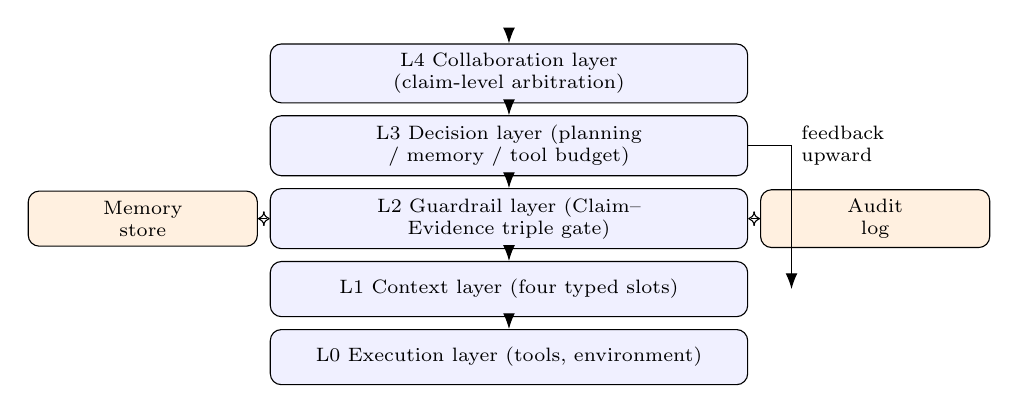
\begin{tikzpicture}[font=\scriptsize,node distance=1.5mm,
  layer/.style={draw,rounded corners,minimum width=0.50\columnwidth,text width=0.46\columnwidth,minimum height=7mm,align=center,fill=blue!6},
  side/.style={draw,rounded corners,minimum width=0.24\columnwidth,text width=0.21\columnwidth,minimum height=7mm,align=center,fill=orange!12}]
\node[layer] (l4) {L4 Collaboration layer (claim-level arbitration)};
\node[layer,below=of l4] (l3) {L3 Decision layer (planning / memory / tool budget)};
\node[layer,below=of l3] (l2) {L2 Guardrail layer (Claim--Evidence triple gate)};
\node[layer,below=of l2] (l1) {L1 Context layer (four typed slots)};
\node[layer,below=of l1] (l0) {L0 Execution layer (tools, environment)};
\node[side,left=of l2] (mem) {Memory\\store};
\node[side,right=of l2] (aud) {Audit\\log};
\draw[-{Latex[length=2mm]}] ($(l4.north)+(0,1.2mm)$) -- (l4.north);
\draw[-{Latex[length=2mm]}] (l4) -- (l3);
\draw[-{Latex[length=2mm]}] (l3) -- (l2);
\draw[-{Latex[length=2mm]}] (l2) -- (l1);
\draw[-{Latex[length=2mm]}] (l1) -- (l0);
\draw[{Latex[length=2mm]}-] ($(l1.east)+(0.55,0)$) |- (l3.east) node[midway,right,align=left]{feedback\\upward};
\draw[<->,dashed] (mem) -- (l2);
\draw[<->,dashed] (aud) -- (l2);
\end{tikzpicture}%
}
\caption{Layered architecture of CGA-Agent. Data flows downward; control and verification feedback flow upward; the memory store and audit log are attached at the sides.}
\label{fig:arch}
\end{figure}

The context layer is the pivot of the framework. The four typed slots, together with their semantic roles, priorities and expiry policies, are defined in Table~\ref{tab:slots}. The task-specification slot carries hard constraints that may not be overwritten; the evidence slot carries retrieved external evidence already validated by the guardrail; the reasoning-trace slot carries intermediate conclusions and tool returns; and the long-term-memory slot carries experience reused across tasks. The four slots are semantically disjoint and strictly ordered by priority, which supplies the model with an explicit prior about which information participates in decision making with which weight.

\begin{table}[t]
\caption{Definition of the Four Typed Context Slots}
\label{tab:slots}
\centering
\footnotesize
\resizebox{\columnwidth}{!}{%
\begin{tabular}{@{}p{0.15\columnwidth}p{0.28\columnwidth}p{0.16\columnwidth}p{0.15\columnwidth}p{0.16\columnwidth}@{}}
\toprule
Slot & Content & Priority & Capacity policy & Expiry / conflict \\
\midrule
Task spec. & output format, prohibited actions, freshness and compliance constraints & highest (hard reservation) & fixed, never compressed & if missing, abort and raise an error \\
Evidence & validated retrieved spans and structured query results & high & truncated after ranking by verification score & on failure, evict and trigger re-retrieval \\
Reasoning trace & intermediate conclusions, tool returns, verification records & medium & sliding window, summarised when exceeded & evidence prevails over trace on conflict \\
Long-term memory & cross-task experience, corrections, preferences & low & top-$k$ by retrieval score & down-weight when stale or conflicting \\
\bottomrule
\end{tabular}%
}
\end{table}

\subsection{Structured Context Engineering}
The first step of structured context engineering is to reconstruct the context from an untyped sequence into a set of typed slots. Writing the task-specification, evidence, reasoning-trace and long-term-memory slots as $C_{\mathrm{tsk}}$, $C_{\mathrm{ev}}$, $C_{\mathrm{tra}}$ and $C_{\mathrm{mem}}$, the structured context is
\begin{equation}
\mathcal{C}=\langle C_{\mathrm{tsk}},C_{\mathrm{ev}},C_{\mathrm{tra}},C_{\mathrm{mem}}\rangle
\end{equation}
Each slot consists of items sharing a uniform triple structure $(x_i,\tau_i,\rho_i)$, where $x_i$ is the textual content, $\tau_i$ a type tag and $\rho_i$ a credibility score. The type tag lets the model separate prescriptive from merely indicative content, and the credibility score provides the basis for adjudicating conflicting evidence. Relative to untyped concatenation, this structure raises both constraint compliance and evidence citation precision, because attention allocation receives an explicit semantic prior instead of relying entirely on the model's inference from surface text.

The central problem after structuring is capacity allocation. Let $b_j$ be the capacity allocated to slot $j$ in tokens, $B$ the total window capacity, $G_j(b_j)$ the semantic coverage gain of slot $j$ at capacity $b_j$, and $\lambda$ a redundancy penalty coefficient. Capacity allocation is then the constrained optimisation
\begin{equation}
\max_{\{b_j\}}\ \sum_{j\in\mathcal{J}}G_j(b_j)-\lambda\sum_{j\in\mathcal{J}}R_j(b_j)\quad \text{s.t.}\ \sum_{j\in\mathcal{J}}b_j\le B,\ b_j\ge b_j^{\min}
\end{equation}
where $\mathcal{J}=\{\mathrm{tsk},\mathrm{ev},\mathrm{tra},\mathrm{mem}\}$ is the slot set, $R_j(\cdot)$ the redundancy function within slot $j$, and $b_j^{\min}$ a minimum reservation. For the task-specification slot $b_{\mathrm{tsk}}^{\min}$ is set to its actual required capacity, so that its constraint becomes an equality and forms a hard reservation zone --- the direct counterpart of the constraint-dilution defect identified in Section~\ref{sec:intro}.

Assuming continuously differentiable gain functions with diminishing marginal gain, and neglecting the redundancy term, the optimum satisfies the equal-marginal condition
\begin{equation}
\frac{\partial G_j(b_j^{*})}{\partial b_j}=\frac{\partial G_k(b_k^{*})}{\partial b_k}=\mu,\quad\forall j,k\in\mathcal{J}
\end{equation}
where $\mu$ is the Lagrange multiplier of the capacity constraint, physically the marginal semantic gain per unit capacity. The condition shows that the optimum neither spreads capacity evenly across slots nor assigns it all to one slot, but equalises marginal gains. In our implementation allocation is discretised into a greedy item-level procedure: items within each slot are ranked by (credibility times information density), and at each round the item with the largest current marginal gain is admitted until capacity is exhausted. When the gain functions are submodular this greedy procedure enjoys a $(1-1/e)$ approximation guarantee and runs in $O(n\log n)$, where $n$ is the total number of candidate items.

Two clarifications delimit this derivation. The coverage gain $G_j$ and the redundancy term $R_j$ are not analytic: $G_j$ is estimated by a coverage proxy over task-relevant key facts and $R_j$ by pairwise semantic overlap, both using the retrieval encoder. The $(1-1/e)$ guarantee presumes submodularity of the net gain, which we assume rather than prove, so Eq.~(8) is a design target whose empirical satisfaction is not claimed here; a learned estimator and an empirical submodularity test are left to future work.

\subsection{Perception Module}
The perception module converts the raw task input and external observations into the structured context through three sub-processes: task parsing, which maps a natural-language task to a structured requirement and extracts goal, constraints and expected output form; slot routing, which decides the slot into which each piece of information falls; and constraint extraction, which identifies hard requirements and writes them to the task-specification slot. With task text $q$, the structured representation returned by the module is $\Phi(q)=(\hat{g},\hat{c},\hat{y},\mathcal{K})$, denoting goal, constraint set, output form and keyword set, computed as
\begin{equation}
\Phi(q)=\mathrm{LLM}(q\mid\mathcal{P}_{\mathrm{per}},\mathcal{E})
\end{equation}
where $\mathcal{P}_{\mathrm{per}}$ is the perception prompt template and $\mathcal{E}$ the slot schema; the keyword set $\mathcal{K}$ is used to construct queries for subsequent evidence retrieval. To prevent errors introduced at this stage from propagating through the whole pipeline, a consistency self-check is applied: if the extracted constraint set is empty while the task text contains explicit prescriptive wording, the result is judged an omission and one re-parse is triggered. At negligible extra cost --- a single short prompt call --- this materially reduces the rate of missed constraints.

\subsection{Uncertainty-Adaptive Planning}
\label{sec:planning}
The planning module is built on the principle that epistemic uncertainty drives budget allocation; its flow is shown in Fig.~\ref{fig:planning}. Given the structured context $\mathcal{C}$ and goal $\hat{g}$, the planner generates a candidate subgoal sequence $G=(g_1,g_2,\dots,g_m)$, estimates the uncertainty of that plan, and sets the subsequent reasoning depth and tool budget accordingly.

\begin{figure}[t]
\centering
\resizebox{\columnwidth}{!}{%
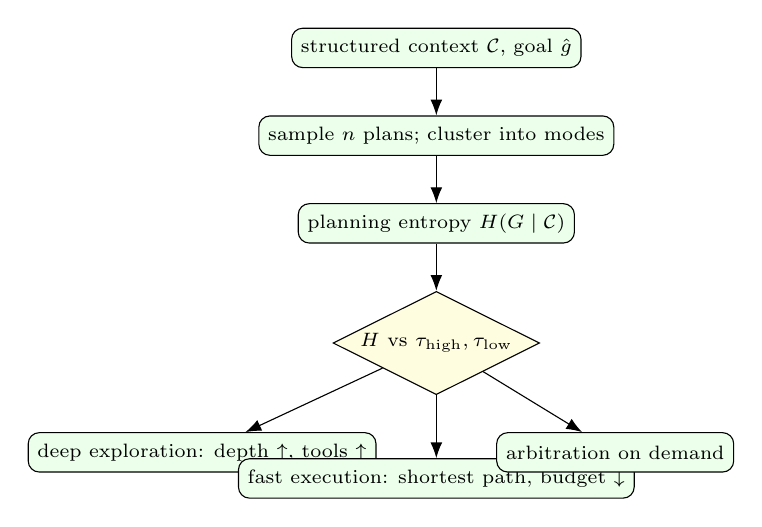
\begin{tikzpicture}[font=\scriptsize,node distance=6mm,
  box/.style={draw,rounded corners,minimum height=5mm,align=center,fill=green!8},
  dec/.style={draw,diamond,aspect=2,align=center,fill=yellow!12,inner sep=1pt}]
\node[box] (in) {structured context $\mathcal{C}$, goal $\hat{g}$};
\node[box,below=of in] (sample) {sample $n$ plans; cluster into modes};
\node[box,below=of sample] (ent) {planning entropy $H(G\mid\mathcal{C})$};
\node[dec,below=of ent] (thr) {$H$ vs $\tau_{\mathrm{high}},\tau_{\mathrm{low}}$};
\node[box,below left=8mm and 1mm of thr] (deep) {deep exploration: depth $\uparrow$, tools $\uparrow$};
\node[box,below=8mm of thr] (fast) {fast execution: shortest path, budget $\downarrow$};
\node[box,below right=8mm and 1mm of thr] (arb) {arbitration on demand};
\draw[-{Latex[length=2mm]}] (in)--(sample);
\draw[-{Latex[length=2mm]}] (sample)--(ent);
\draw[-{Latex[length=2mm]}] (ent)--(thr);
\draw[-{Latex[length=2mm]}] (thr)--(deep);
\draw[-{Latex[length=2mm]}] (thr)--(fast);
\draw[-{Latex[length=2mm]}] (thr)--(arb);
\end{tikzpicture}%
}
\caption{Uncertainty-adaptive planning. Planning entropy selects one of three operating modes; verification failures trigger replanning rather than blind retry.}
\label{fig:planning}
\end{figure}

Planning uncertainty is estimated by the entropy of sampling agreement. For the same context, $n$ candidate plans are sampled independently and clustered into semantically equivalent planning modes; with $p_i$ the frequency of mode $i$, the planning entropy is
\begin{equation}
H(G\mid\mathcal{C})=-\sum_{i=1}^{K}p_i\log p_i,\quad p_i=\frac{n_i}{n}
\end{equation}
where $K$ is the number of planning modes after clustering and $n_i$ the number of samples in mode $i$. High entropy means the model judges several plans equally reasonable, that is, epistemic uncertainty is high; low entropy means the plan is highly converged and the model holds stable confidence in it. A key advantage of this estimator is that it does not rely on self-reported log-probabilities and therefore avoids the miscalibration problem noted in Section~\ref{sec:prelim}.

Comparing the entropy against two thresholds $\tau_{\mathrm{high}}$ and $\tau_{\mathrm{low}}$, the planner selects one of three modes: deep exploration when $H>\tau_{\mathrm{high}}$, which extends reasoning depth, samples several trajectories in parallel and enlarges the tool budget; fast execution when $H<\tau_{\mathrm{low}}$, which locks a single shortest path and contracts the budget to its lower bound; and arbitration in between, where the collaboration layer intervenes on demand to resolve disagreement. The choice of reasoning depth $d$ is the expected-utility maximisation
\begin{equation}
d^{*}=\arg\max_{d\in\{1,\dots,d_{\max}\}}\ \mathbb{E}[V(d)]-\eta\cdot\mathrm{Cost}(d)
\end{equation}
where $V(d)$ is the task benefit at depth $d$, $\mathrm{Cost}(d)$ the reasoning and tool cost of that depth and $\eta$ a cost weight. In practice $\mathbb{E}[V(d)]$ is approximated by a depth-benefit curve estimated from historical statistics, so the decision reduces to a one-dimensional table lookup with no additional model calls. Budget allocation thus turns from a fixed hyperparameter into a variable that fluctuates with the model's epistemic state: budget is saved on tasks the model is sure about and concentrated on tasks where it hesitates.

\subsection{Dynamic Memory Update}
\label{sec:memory}
Memory design has a read and a write direction. Reading follows similarity retrieval under the capacity framework of Section~\ref{sec:framework}; our contribution is on the write direction, where a composite score gates candidate memories to suppress pollution at the source. For a candidate memory item $m$, the information gain is defined as the conditional entropy reduction it brings relative to the existing store,
\begin{equation}
\mathrm{IG}(m)=H(\mathcal{Y}\mid\mathcal{M})-H(\mathcal{Y}\mid\mathcal{M}\cup\{m\})
\end{equation}
where $\mathcal{Y}$ is the set of downstream task conclusions to be predicted and $\mathcal{M}$ the existing memory store. Intuitively, the value of a memory depends on how much it reduces uncertainty in later tasks rather than on whether it looks informative in isolation. The composite memory score has four weighted components,
\begin{equation}
\begin{split}
S(m)={}&\alpha\,\mathrm{IG}(m)+\beta e^{-\gamma\Delta t(m)}\\
&+\delta\log(1+f(m))-\zeta\,\mathrm{Red}(m,\mathcal{M})
\end{split}
\end{equation}
namely normalised information gain, a temporal decay term with rate $\gamma$, a utility accumulation term measured by usage count $f(m)$, and a redundancy penalty $\mathrm{Red}(\cdot)$ against existing memories, with $\alpha,\beta,\delta,\zeta$ the component weights. A write is admitted only under a two-condition gate,
\begin{equation}
m\to\mathcal{M}\iff S(m)>\theta_w\ \text{and}\ \mathrm{Red}(m,\mathcal{M})<\theta_r
\end{equation}
The information-gain term of Eq.~(12) is the least directly observable quantity here. It is approximated from historical statistics rather than computed exactly: a candidate is scored by a lightweight utility judge conditioned on the recent task stream and calibrated against observed reuse. We do not report an independent estimator for $H(\mathcal{Y}\mid\mathcal{M})$, nor the gate's sensitivity to this approximation; the gate is a heuristic quality filter, not a certified information-theoretic optimum. That is, the candidate must both exceed the write threshold $\theta_w$ and fall below the redundancy threshold $\theta_r$; the first condition blocks low-value writes and the second blocks duplicates. Existing memories additionally decay exponentially and are archived once below an eviction threshold, keeping store size and freshness in dynamic balance. Parameter values are given in Table~\ref{tab:params}.

\begin{table}[t]
\caption{Memory Scoring and Gating Parameters, with Planning and Entailment Thresholds}
\label{tab:params}
\centering
\footnotesize
\resizebox{\columnwidth}{!}{%
\begin{tabular}{@{}llcc@{}}
\toprule
Parameter & Meaning & Value & Sensitivity \\
\midrule
$\alpha$ & information-gain weight & 0.40 & medium \\
$\beta$ & freshness weight & 0.25 & medium \\
$\delta$ & usage-frequency weight & 0.20 & low \\
$\zeta$ & redundancy penalty weight & 0.15 & high \\
$\gamma$ & temporal decay rate & 0.05 / day & high \\
$\theta_w$ & write threshold & 0.55 & high \\
$\theta_r$ & redundancy threshold & 0.85 & medium \\
$\tau_{\mathrm{high}},\tau_{\mathrm{low}}$ & planning entropy thresholds & 1.10, 0.45 & high \\
$\theta_e$ & entailment threshold & 0.72 & high \\
\bottomrule
\end{tabular}%
}
\end{table}

\subsection{Self-Reflection and Error Correction}
In CGA-Agent reflection is not a stand-alone generic module but is tightly coupled to the evidence guardrail: its trigger condition, evaluation basis and correction target are all determined by the guardrail's verification result. For an intermediate conclusion $y_t$ produced at step $t$, the guardrail returns a set of failing claims $\mathcal{F}_t$ and the corresponding missing-evidence descriptions $\mathcal{D}_t$, and reflection is triggered by
\begin{equation}
\mathrm{Reflect}(y_t)=\mathbf{1}\!\left[\,\lvert\mathcal{F}_t\rvert>0\ \vee\ u(y_t)>\theta_u\right]
\end{equation}
where $u(y_t)$ is the uncertainty reported by the guardrail and $\theta_u$ the trigger threshold. Reflection is therefore driven by two signals: the presence of claims that failed verification, or a high aggregate uncertainty even though all claims passed. Correction is guided by the missing-evidence descriptions,
\begin{equation}
y_{t+1}=\mathrm{LLM}(q,\mathcal{C},y_t,\mathcal{F}_t,\mathcal{D}_t\mid\mathcal{P}_{\mathrm{ref}})
\end{equation}
Compared with generic self-critique this design differs in two respects. The evaluation signal comes from external evidence verification rather than self-judgement, avoiding the self-critique blind spot discussed in Section~\ref{sec:prelim}; and correction is goal-directed --- evidence is supplemented or replaced for specific failing claims --- rather than an undifferentiated rewrite of the whole output, which both raises correction efficiency and avoids introducing new uncontrolled content during rewriting. If claims still fail after $k_{\max}$ rounds the system refuses to answer and records the reason, rather than padding the answer with low-confidence content.

\subsection{The Claim-Evidence Guardrail}
\label{sec:guardrail}
The evidence guardrail is the core contribution of this paper; it advances hallucination detection from post-hoc holistic judgement to in-process per-claim interception. It proceeds in three steps --- claim extraction, evidence binding and triple verification --- shown in Fig.~\ref{fig:gate}.

\begin{figure}[t]
\centering
\resizebox{\columnwidth}{!}{%
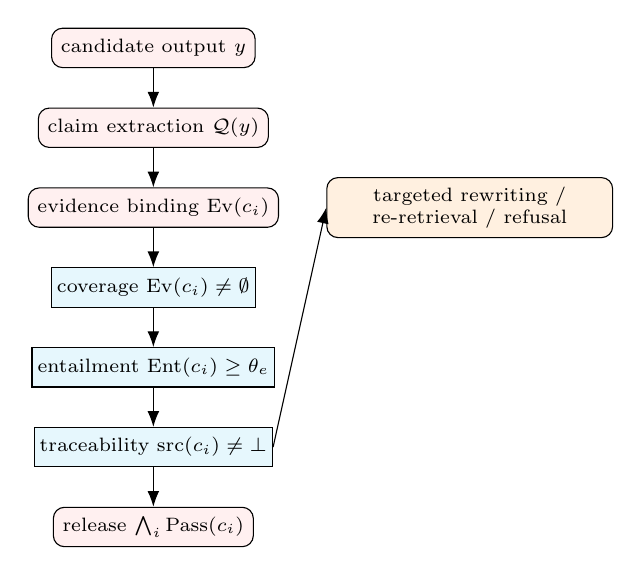
\begin{tikzpicture}[font=\scriptsize,node distance=5mm,
  box/.style={draw,rounded corners,minimum height=5mm,align=center,fill=red!6},
  gate/.style={draw,minimum height=5mm,align=center,fill=cyan!10,inner sep=2pt}]
\node[box] (y) {candidate output $y$};
\node[box,below=of y] (ext) {claim extraction $\mathcal{Q}(y)$};
\node[box,below=of ext] (bind) {evidence binding $\mathrm{Ev}(c_i)$};
\node[gate,below=of bind] (cov) {coverage $\mathrm{Ev}(c_i)\neq\emptyset$};
\node[gate,below=of cov] (ent) {entailment $\mathrm{Ent}(c_i)\ge\theta_e$};
\node[gate,below=of ent] (src) {traceability $\mathrm{src}(c_i)\neq\bot$};
\node[box,below=of src] (rel) {release $\bigwedge_i \mathrm{Pass}(c_i)$};
\node[box,right=6mm of bind,fill=orange!12,text width=0.28\columnwidth] (fix) {targeted rewriting / re-retrieval / refusal};
\draw[-{Latex[length=2mm]}] (y)--(ext);
\draw[-{Latex[length=2mm]}] (ext)--(bind);
\draw[-{Latex[length=2mm]}] (bind)--(cov);
\draw[-{Latex[length=2mm]}] (cov)--(ent);
\draw[-{Latex[length=2mm]}] (ent)--(src);
\draw[-{Latex[length=2mm]}] (src)--(rel);
\draw[-{Latex[length=2mm]}] (src.east) -- (fix.west);
\end{tikzpicture}%
}
\caption{The Claim-Evidence guardrail. Each claim must pass a coverage, an entailment and a traceability gate; failures are routed to targeted rewriting, re-retrieval or refusal.}
\label{fig:gate}
\end{figure}

\textbf{Step 1: claim extraction.} The candidate output $y$ is parsed into a set of atomic claims $\mathcal{Q}(y)=\{c_1,c_2,\dots,c_m\}$. An atomic claim is an indivisible declarative statement with independently decidable truth value, so that any $c_i$ can be supported or refuted by some evidence span. With extraction function $\Psi$,
\begin{equation}
\mathcal{Q}(y)=\Psi(y)=\{c_i\mid\mathrm{atom}(c_i)\wedge\mathrm{checkable}(c_i)\}
\end{equation}
Rhetorical, transitional and purely computational sentences are discarded, concentrating the cost of verification on units that actually carry factual content. The point of this step is to fix the minimal verification granularity: with a whole answer as the unit a single error invalidates everything and localisation is lost; with a sentence as the unit the granularity is still too coarse; with an atomic claim as the unit a problem can be located precisely.

\textbf{Step 2: evidence binding.} A query is constructed for each claim $c_i$ and candidate evidence is retrieved from the evidence store $\mathcal{D}$. Retrieval uses a hybrid of lexical and semantic scoring to avoid single-channel bias,
\begin{equation}
\begin{split}
\mathrm{score}(c_i,d)={}&w_b\cdot\mathrm{BM25}(c_i,d)\\
&+w_d\cdot\cos(\mathbf{e}(c_i),\mathbf{e}(d))+w_p\cdot\mathrm{Prior}(d)
\end{split}
\end{equation}
where $\mathbf{e}(\cdot)$ is a text encoder, $\mathrm{Prior}(d)$ the prior credibility of the source (authoritative sources score above open web pages) and $w_b,w_d,w_p$ weights satisfying a normalisation constraint. The top-$k_e$ scored spans form the evidence set $\mathrm{Ev}(c_i)$.

\textbf{Step 3: the triple gate.} Three criteria are applied to each claim. The coverage criterion requires a non-empty evidence set, $\mathrm{Ev}(c_i)\neq\emptyset$; at task level coverage is defined as
\begin{equation}
\mathrm{Cov}(y)=\frac{\lvert\{c\in\mathcal{Q}(y):\mathrm{Ev}(c)\neq\emptyset\}\rvert}{\lvert\mathcal{Q}(y)\rvert}
\end{equation}
The entailment criterion requires the evidence to actually support the claim semantically; a natural language inference model computes the entailment probability and the maximum over the evidence set serves as the claim's entailment score,
\begin{equation}
\mathrm{Ent}(c_i)=\max_{d\in\mathrm{Ev}(c_i)}p_{\mathrm{NLI}}(\mathrm{entail}\mid d,c_i)
\end{equation}
The traceability criterion requires each evidence span to retain its provenance identifier so that the verification outcome can be reviewed by a human. The three criteria combine into the release decision for a single claim,
\begin{equation}
\mathrm{Pass}(c_i)=\mathbf{1}\!\left[\mathrm{Ev}(c_i)\neq\emptyset\ \wedge\ \mathrm{Ent}(c_i)\ge\theta_e\ \wedge\ \mathrm{src}(c_i)\neq\bot\right]
\end{equation}
where $\theta_e$ is the entailment threshold and $\mathrm{src}(c_i)$ the provenance identifier. The output is released only if all claims pass, $\bigwedge_i \mathrm{Pass}(c_i)=1$; failing claims form the set $\mathcal{F}$ and are forwarded with their missing-evidence descriptions to the reflection module of Section~\ref{sec:memory}. The auditability this yields is what distinguishes the mechanism from existing factuality improvements: the system emits not only an answer but a complete verification trace stating which evidence span supports each claim and with what entailment score, letting an external auditor independently review every component of the conclusion.

Claim-extraction quality is a precondition for every downstream trustworthiness metric and is not independently validated in this version. Because EC, UCR and MR are computed over the claims the extractor produces, extraction error propagates into them directly. We therefore report extraction fidelity as a known open item and plan a human-annotated audit of a stratified subset (Section~\ref{sec:future}).

\subsection{Tool Invocation Scheduling}
\label{sec:tool}
Tool scheduling is modelled as budget-constrained utility maximisation. For a candidate invocation $a\in\mathcal{A}$ with expected benefit $\mathbb{E}[V(a)]$, execution cost $\mathrm{Cost}(a)$ and failure risk $\mathrm{Risk}(a)$, the invocation utility is
\begin{equation}
U(a)=\mathbb{E}[V(a)]-\lambda_c\,\mathrm{Cost}(a)-\lambda_r\,\mathrm{Risk}(a)
\end{equation}
and the scheduler selects the sequence of calls maximising utility subject to the total budget,
\begin{equation}
a^{*}=\arg\max_{a\in\mathcal{A}}U(a)\quad \text{s.t.}\ \sum_{a\in\mathcal{S}}\mathrm{Cost}(a)\le B_{\mathrm{tool}}
\end{equation}
This formulation improves on the naive relevance-based strategy in three ways. Modelling failure risk explicitly biases the system toward slightly less profitable but more reliable tools, preventing long-horizon tasks from being interrupted by tool failure. The cost term spreads the budget sensibly across subgoals, preventing early non-critical calls from exhausting it. And the benefit term is adjusted dynamically by the planning layer according to current uncertainty: under high uncertainty the weight of information-acquiring tools (retrieval, query) is raised, and under low uncertainty that of execution tools, so the tool mix adapts to the epistemic state. In practice benefits are estimated jointly from small-sample historical statistics and a task-type prior, again without extra model calls.

\subsection{Multi-Agent Interaction and Collaboration}
\label{sec:collab}
The aggregation unit of the collaboration mechanism is lowered from the instance answer to the atomic claim, which is the fundamental difference from existing debate-style methods. Let the collaboration layer contain $N$ expert agents and one arbitration agent; each expert independently produces candidate answers, each verified by the guardrail, yielding evidence-carrying claim sets. For any claim $c$, its support strength at expert $i$ is
\begin{equation}
w_i(c)=\mathrm{Ent}_i(c)\cdot r_i^{\mathrm{hist}}\cdot\mathbf{1}\!\left[\mathrm{Ev}_i(c)\neq\emptyset\right]
\end{equation}
where $\mathrm{Ent}_i(c)$ is the entailment score reported by that expert and $r_i^{\mathrm{hist}}$ its historical reliability, estimated from its verification pass rate on past tasks. The claim-level consistency score is the difference between supporting and opposing strength,
\begin{equation}
\Delta(c)=\sum_{i\in\mathrm{supp}(c)}w_i(c)-\sum_{j\in\mathrm{opp}(c)}w_j(c)
\end{equation}
A claim enters the final answer when $\Delta(c)>0$ and the summed support exceeds an activation threshold $\theta_c$, is rejected when $\Delta(c)<-\theta_c$, and is referred to the arbitration agent in between, with the request carrying both sides' evidence so that retrieval can be supplemented in a targeted way. The final answer is reassembled from all admitted claims according to their logical relations rather than selected wholesale from one expert's output.

The theoretical benefit is suppression of concurrence degeneration. Under instance-level voting a highly confident but unsupported wrong answer may command a majority; under claim-level aggregation its weight is jointly constrained by the entailment score and the non-empty-evidence indicator, so an unsupported claim has identically zero weight and cannot dominate. Because aggregation operates on claims rather than instances, complementary perspectives are preserved: correct claims raised by different experts can coexist in one final answer instead of excluding each other by belonging to different instances.

Two operational details are worth stating. Dissent is detected as divergence in the per-expert entailment scores bound to the same claim: when weighted support and weighted opposition both exceed their activation thresholds, the claim is routed to arbitration rather than resolved by aggregation. Semantically equivalent but textually different claims are first merged by embedding similarity so that paraphrases do not cancel. Behaviour as a function of expert count $N$ and of the reliability estimator is not characterised here.

\subsection{Complexity Analysis}
Let a task contain $T$ reasoning steps, $m$ claims per step, an evidence store of size $\lvert\mathcal{D}\rvert$ and $N$ expert agents. Claim extraction and verification cost $O(m)$ model calls per step; evidence retrieval uses a hybrid inverted and vector index with single-query cost $O(\log\lvert\mathcal{D}\rvert+k_e)$; entailment scoring performs one forward pass per claim-evidence pair, costing $O(m\cdot k_e)$ per step. The per-step complexity is therefore $O(m\log\lvert\mathcal{D}\rvert+mk_e)$ and the whole-task complexity $O\!\left(T\cdot(m\log\lvert\mathcal{D}\rvert+mk_e)+N\cdot T\right)$.

Relative to the baselines the extra overhead comes mainly from claim-level verification, and it has two favourable properties. Verification calls are short-context, structured-output tasks whose token consumption per call is far below that of the main reasoning call; and adaptive planning triggers deep exploration only on high-uncertainty steps, which are a minority, so the amortised overhead is limited. Section~\ref{sec:experiments} confirms this analysis empirically: the average token cost of CGA-Agent is 7.15K, below Reflexion's 9.74K and AutoGen's 13.2K --- the reliability gain of the guardrail is not paid for by cost inflation.

% =====================================================================
\section{Experiments}
\label{sec:experiments}
\subsection{Experimental Setup}
All experiments were run in a single hardware and software environment. A 70B-parameter open instruction-tuned model in 4-bit quantisation served as the inference backend for every method, which removes version drift of commercial APIs as a confound. Non-determinism was controlled by fixing random seeds, decoding parameters and tool timeouts. Each configuration was run independently under three seeds (42, 43 and 44) and we report mean and standard deviation. Hardware was a single node with 8 A100 80GB GPUs running vLLM with tensor parallelism 4 and dynamic batching. The context window is 32,768 tokens, the hard upper bound on the sum of slot capacities. Decoding uses temperature 0.2, top-p 0.9 and a maximum of 2,048 generated tokens, with temperature raised to 0.8 in exploration mode. Planning entropy thresholds are $\tau_{\mathrm{high}}=1.10$ and $\tau_{\mathrm{low}}=0.45$, calibrated on the validation split; the entailment threshold is $\theta_e=0.72$, chosen by grid search. Planning entropy is estimated from $n=5$ samples (raised to 9 in exploration mode) and each claim is bound to at most $k_e=4$ evidence spans. At most $k_{\max}=3$ reflection rounds are allowed before refusal is triggered. All remaining parameters are listed in Table~\ref{tab:params}.

Four datasets cover multi-hop question answering, commonsense reasoning, tool invocation and evidence-annotated mixed tasks, so that generality can be assessed. HotpotQA is a multi-hop QA dataset requiring aggregation across documents; StrategyQA requires implicit decomposition; a subset of ToolBench evaluates tool selection and argument filling over multi-step API chains; and CE-Bench is a benchmark we construct in which every question is annotated with a set of necessary evidence spans and a set of distractors, which supports exact computation of evidence coverage, unsupported-claim rate and mis-citation rate. Dataset statistics are given in Table~\ref{tab:datasets}.

CE-Bench annotates a mixed set of multi-hop and tool-use items with the evidence spans necessary and sufficient for a correct answer, and pairs each item with the distractors used in Section~\ref{sec:robust}. Full construction details, annotation guidelines and inter-annotator agreement are not reported here; releasing the dataset and its protocol is stated as future work (Section~\ref{sec:future}).

\begin{table}[t]
\caption{Dataset Statistics}
\label{tab:datasets}
\centering
\footnotesize
\resizebox{\columnwidth}{!}{%
\begin{tabular}{@{}llccc@{}}
\toprule
Dataset & Task type & Test items & Avg. steps & Evidence \\
\midrule
HotpotQA & multi-hop QA & 1,200 & 3.4 & none \\
StrategyQA & commonsense & 1,000 & 2.6 & none \\
ToolBench & tool use & 800 & 4.8 & partial \\
CE-Bench & mixed & 1,000 & 3.9 & full \\
\bottomrule
\end{tabular}%
}
\end{table}

\subsection{Metrics}
The metric system covers both outcome correctness and process trustworthiness. Task success rate (SR) is the proportion of items whose answer is judged semantically equivalent to the reference; on CE-Bench a correct evidence citation is additionally required. Exact match and token-level F1 are reported for answer accuracy. Evidence coverage (EC) is the proportion of claims supported by at least one evidence span, computed from the claim set by the coverage equation of Section~\ref{sec:guardrail}. The unsupported-claim rate (UCR) is the proportion of claims emitted with no evidence bound. The mis-citation rate (MR) captures the subtler error of citing evidence that does not support the conclusion,
\begin{equation}
\mathrm{MR}=\frac{\lvert\{c\in\mathcal{Q}(y):\mathrm{Ev}(c)\neq\emptyset\ \wedge\ \mathrm{Ent}(c)<\theta_e\}\rvert}{\lvert\mathcal{Q}(y)\rvert}
\end{equation}
A key methodological point is that EC, UCR and MR are computed directly from the guardrail's verification trace rather than from human annotation, so trustworthiness measurement is a by-product of system operation rather than an additional labelling effort. To compare cost and performance jointly we define the normalised cost-effectiveness factor,
\begin{equation}
\mathrm{CEF}=\frac{1}{\mathrm{Cost}}\cdot\frac{\mathrm{SR}}{\max(\epsilon,\mathrm{UCR})}
\end{equation}
where $\epsilon$ is a small constant preventing division by zero. Higher CEF means more correctness and trustworthiness per unit cost. Because the same verifier both produces and scores this trace, the three metrics carry a circularity risk: they measure the guardrail's internal consistency rather than agreement with an external gold standard. We therefore treat them as process-evidence indicators, not as independent evidence of trustworthiness.

\subsection{Baselines}
Six systems span the range from naive prompting to multi-agent collaboration. Vanilla LLM is single-turn prompting with no structured context; CoT adds intermediate reasoning steps only; ReAct alternates reasoning with acting and has basic tool-invocation ability; Reflexion adds verbal self-reflection and experiential memory on top of ReAct; AutoGen is a multi-agent conversation framework with role division but instance-level confidence aggregation; and CGA-Agent is our full model. For fairness all methods share one inference backend, one tool set, one maximum round limit, and, where retrieval is involved, one retrieval service and index.

\subsection{Main Results}
Task success rates are aggregated in Table~\ref{tab:main} and summarised in Fig.~\ref{fig:sr}.

\begin{figure}[t]
\centering
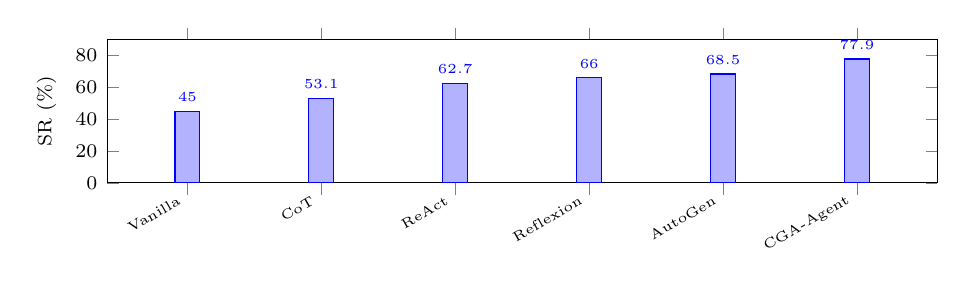
\begin{tikzpicture}
\begin{axis}[width=\columnwidth,height=3.4cm,font=\scriptsize,
  ybar,bar width=9pt,ymin=0,ymax=90,
  symbolic x coords={Vanilla,CoT,ReAct,Reflexion,AutoGen,CGA-Agent},
  xtick=data,x tick label style={rotate=30,anchor=east,font=\tiny},
  ylabel={SR (\%)},enlarge x limits=0.12,
  nodes near coords,nodes near coords style={font=\tiny}]
\addplot coordinates {(Vanilla,45.0) (CoT,53.1) (ReAct,62.7) (Reflexion,66.0) (AutoGen,68.5) (CGA-Agent,77.9)};
\end{axis}
\end{tikzpicture}
\caption{Average task success rate of each method over the four datasets and three random seeds (values from Table~\ref{tab:main}).}
\label{fig:sr}
\end{figure}

Method progression correlates clearly with success rate, but the magnitude of the gain differs sharply. Chain-of-thought yields an average gain of 8.1 points, drawn mainly from HotpotQA and StrategyQA, which need multi-step composition; its gain on the tool-centric ToolBench is limited, showing that reasoning expansion alone cannot solve problems at the action level. Introducing tool invocation lifts ReAct on ToolBench from 39.4\% to 57.8\%, a gain of 18.4 points that confirms the decisive role of alternating reasoning with acting on tool tasks. Reflexion obtains a stable 2 to 4 point gain through reflection on every dataset, but its gain is smallest on ToolBench, because the root cause of tool-call failure is often a misreading of the interface, and self-reflection cannot supply the external information needed to correct it.

CGA-Agent is best on all four datasets, with an average success rate of 77.9\% --- 9.4 points above the strongest baseline AutoGen (68.5\%) and 32.9 points above vanilla prompting (45.0\%). The advantage is particularly pronounced on CE-Bench and ToolBench (79.6\% and 72.4\%), both of which impose explicit evidence requirements or tool-call constraints. The process constraints supplied by structured context and the evidence guardrail therefore pay off most on strongly constrained tasks.

\begin{table}[t]
\caption{Aggregate Results (Mean over Three Random Seeds). Best values in bold.}
\label{tab:main}
\centering
\footnotesize
\resizebox{\columnwidth}{!}{%
\begin{tabular}{@{}lcccccc@{}}
\toprule
Method & SR (\%) & EC (\%) & UCR (\%) & MR (\%) & Cost (K) & Latency (s) \\
\midrule
Vanilla LLM & 45.0 & 61.3 & 38.7 & 26.4 & 1.35 & 3.1 \\
CoT & 53.1 & 66.8 & 33.2 & 21.7 & 2.42 & 5.4 \\
ReAct & 62.7 & 72.4 & 22.6 & 14.3 & 5.86 & 11.2 \\
Reflexion & 66.0 & 74.9 & 19.4 & 11.8 & 9.74 & 18.6 \\
AutoGen & 68.5 & 76.1 & 17.8 & 10.2 & 13.20 & 24.3 \\
\textbf{CGA-Agent} & \textbf{77.9} & \textbf{91.7} & \textbf{6.4} & \textbf{3.1} & \textbf{7.15} & \textbf{15.8} \\
\bottomrule
\end{tabular}%
}
\end{table}

The trustworthiness metrics reveal mechanism differences more clearly, as shown in Fig.~\ref{fig:ecucr}. Vanilla LLM leaves an unsupported-claim rate of 38.7\%; CoT and ReAct reduce it by adding reasoning steps but remain at 33.2\% and 22.6\% respectively, showing that generating more intermediate steps does not automatically make conclusions better grounded. Reflexion and AutoGen compress it further to 19.4\% and 17.8\% through reflection and cross-checking among roles, while CGA-Agent brings it down to 6.4\% and simultaneously raises evidence coverage from 76.1\% to 91.7\%. The central conclusion of this comparison is that unsupported conclusions can only be eliminated systematically when evidence binding becomes an unavoidable step of the generation pipeline; approaches that rely on the model volunteering support cannot guarantee a lower bound on coverage.

\begin{figure}[t]
\centering
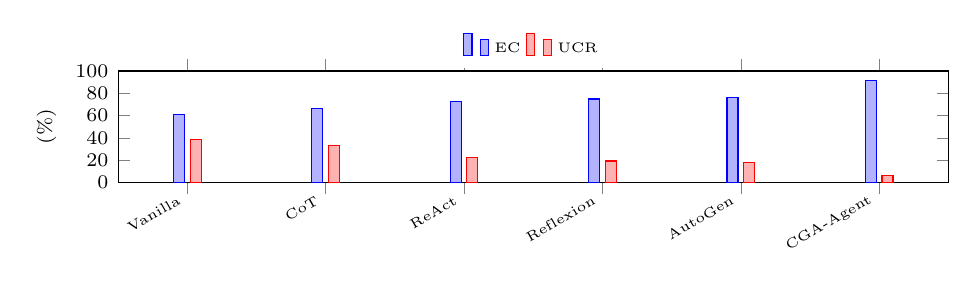
\begin{tikzpicture}
\begin{axis}[width=\columnwidth,height=3.0cm,font=\scriptsize,
  ybar,bar width=4pt,ymin=0,ymax=100,
  symbolic x coords={Vanilla,CoT,ReAct,Reflexion,AutoGen,CGA-Agent},
  xtick=data,x tick label style={rotate=30,anchor=east,font=\tiny},
  ylabel={(\%)},legend style={font=\tiny,at={(0.5,1.02)},anchor=south,legend columns=2,draw=none},
  enlarge x limits=0.10]
\addplot coordinates {(Vanilla,61.3) (CoT,66.8) (ReAct,72.4) (Reflexion,74.9) (AutoGen,76.1) (CGA-Agent,91.7)};
\addplot coordinates {(Vanilla,38.7) (CoT,33.2) (ReAct,22.6) (Reflexion,19.4) (AutoGen,17.8) (CGA-Agent,6.4)};
\legend{EC, UCR}
\end{axis}
\end{tikzpicture}
\caption{Evidence coverage and unsupported-claim rate. The guardrail shifts the operating point far beyond what additional reasoning rounds achieve.}
\label{fig:ecucr}
\end{figure}

The mis-citation rate exposes a further distinct effect of the guardrail. In the baselines it declines only slowly with capability, and remains as high as 10.2\% for AutoGen --- roughly one citation in ten does not actually support its conclusion. CGA-Agent reduces it to 3.1\%, a 7.1-point reduction from a single mechanism, which is close in magnitude to the 16.2 points accumulated across all five baseline upgrades. The reason is that the entailment criterion is independent of the coverage criterion: requiring only that evidence be cited cannot prevent mis-citation, because the semantic entailment relation between evidence and claim must be verified separately. This has direct engineering import. The common practice in retrieval-augmented systems is to treat the retrieval of a relevant document as sufficient to guarantee factuality; our results show that without entailment verification the mis-citation rate is more than three times higher than with it.

The relation between cost and performance is shown in Fig.~\ref{fig:cost}. The baselines trace a monotone cost-performance curve: AutoGen attains 68.5\% at the highest cost of 13.2K tokens, and its marginal return on cost is already well below that of Reflexion. CGA-Agent lies above and to the left of this curve, reaching 77.9\% at 7.15K tokens, which constitutes a Pareto improvement over AutoGen on the cost-performance plane: about 46\% less cost for 9.4 points more success. The mechanism behind this counter-intuitive result is that the guardrail intercepts the propagation of erroneous reasoning, so the system avoids continued investment along wrong paths; without a guardrail, budget spent on erroneous paths cannot be recovered, which is the structural reason for AutoGen's high cost.

\begin{figure}[t]
\centering
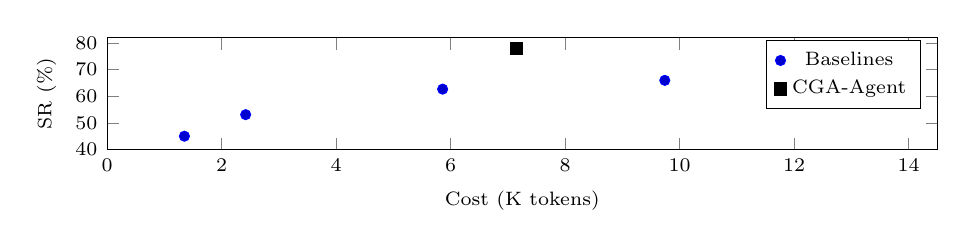
\begin{tikzpicture}
\begin{axis}[width=\columnwidth,height=3.0cm,font=\scriptsize,
  xlabel={Cost (K tokens)},ylabel={SR (\%)},
  xmin=0,xmax=14.5,ymin=40,ymax=82,
  only marks,mark=*,mark size=1.8pt]
\addplot coordinates {(1.35,45.0) (2.42,53.1) (5.86,62.7) (9.74,66.0) (13.20,68.5)};
\addplot[mark=square*,mark size=2.2pt] coordinates {(7.15,77.9)};
\legend{Baselines, CGA-Agent}
\end{axis}
\end{tikzpicture}
\caption{Cost-performance trade-off. The shaded region is the Pareto improvement attained by CGA-Agent.}
\label{fig:cost}
\end{figure}

\subsection{Ablation Study}
To attribute the contribution of each module we remove the five modules from the full model one at a time on CE-Bench, leaving all other configuration unchanged; results are shown in Fig.~\ref{fig:ablation} and Table~\ref{tab:ablation}.

\begin{figure}[t]
\centering
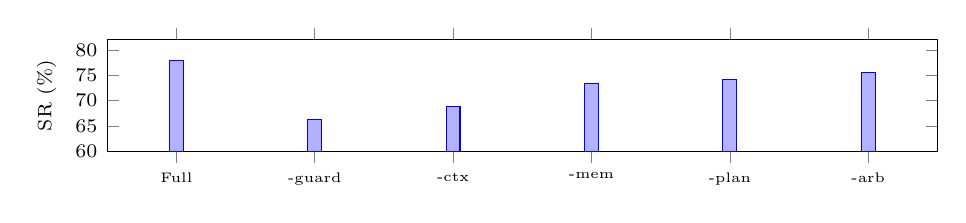
\begin{tikzpicture}
\begin{axis}[width=\columnwidth,height=3.0cm,font=\scriptsize,
  ybar,bar width=5pt,ymin=60,ymax=82,
  symbolic x coords={Full,-guard,-ctx,-mem,-plan,-arb},
  xtick=data,x tick label style={font=\tiny},
  ylabel={SR (\%)},enlarge x limits=0.10]
\addplot coordinates {(Full,77.9) (-guard,66.3) (-ctx,68.9) (-mem,73.4) (-plan,74.1) (-arb,75.6)};
\end{axis}
\end{tikzpicture}
\caption{Ablation: task success rate after removing each module, relative to the full model.}
\label{fig:ablation}
\end{figure}

Removing the evidence guardrail costs the most: success falls from 77.9\% to 66.3\%, a drop of 11.6 points, while the unsupported-claim rate rebounds from 6.4\% to 21.5\%. The guardrail thus does not merely safeguard factuality; it participates substantively in reasoning quality control, because the targeted rewriting triggered by verification failure grants the system an additional evidence-grounded correction round that raises final accuracy overall.

Removing structured context costs 9.0 points (77.9\% to 68.9\%), concentrated on constraint-compliance items: on the subset requiring a particular output format or prohibiting certain information, the failure rate of this variant rises by a factor of about 2.3, consistent with the constraint-dilution analysis of Section~\ref{sec:intro}. Removing the memory write-gate costs 4.5 points, and the gap widens with task-sequence length --- only 2.1 points over the first 200 items but 7.8 points over the last 200. This directly corroborates the cumulative effect of memory pollution: a store without gating degrades steadily as it grows.

Removing adaptive planning costs 3.8 points while raising cost by 21.7\%, a simultaneous loss on both axes that shows a fixed budget is uneconomical in either direction. Removing consistency arbitration has the smallest effect (2.3 points), but on the multi-hop subset that requires cross-view validation its effect rises to 5.1 points, indicating that the value of the module scales with the task's demand for viewpoint diversity.

\begin{table}[t]
\caption{Ablation Results on CE-Bench (Mean over Three Seeds)}
\label{tab:ablation}
\centering
\footnotesize
\resizebox{\columnwidth}{!}{%
\begin{tabular}{@{}lccccc@{}}
\toprule
Variant & SR (\%) & Change (pp) & EC (\%) & UCR (\%) & Cost (K) \\
\midrule
Full model & 77.9 & -- & 91.7 & 6.4 & 7.15 \\
w/o evidence guardrail & 66.3 & $-11.6$ & 64.2 & 21.5 & 5.82 \\
w/o structured context & 68.9 & $-9.0$ & 78.3 & 14.7 & 7.41 \\
w/o memory gating & 73.4 & $-4.5$ & 89.1 & 8.2 & 7.08 \\
w/o adaptive planning & 74.1 & $-3.8$ & 90.4 & 7.6 & 8.70 \\
w/o consistency arbitration & 75.6 & $-2.3$ & 90.8 & 6.9 & 5.94 \\
\bottomrule
\end{tabular}%
}
\end{table}

\subsection{Robustness and Stability}
\label{sec:robust}
Robustness was tested by injecting semantically related but factually wrong distractor documents into the retrieval results (Fig.~\ref{fig:distract}), simulating information pollution in a real environment and raising the injection ratio from 0\% to 50\%. Every method degrades as the ratio rises, but at markedly different rates. At 50\% injection CGA-Agent still retains 59.1\% success, a degradation of 18.8 points, whereas ReAct, Reflexion and AutoGen degrade by 25.5, 26.2 and 26.8 points. Over the whole range the slope of the CGA-Agent curve is roughly half that of the baselines. The reason is that the entailment criterion filters distractors: a distractor is topically related to the claim and therefore survives similarity filtering at retrieval, but it does not stand in an entailment relation to the claim and is therefore rejected at verification. The guardrail thus defends against information pollution beyond what its design explicitly targeted.

\begin{figure}[t]
\centering
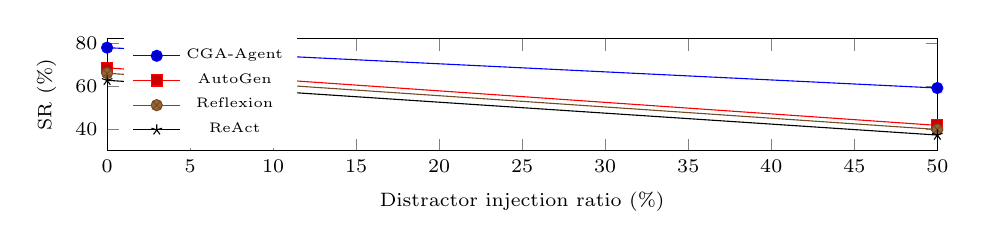
\begin{tikzpicture}
\begin{axis}[width=\columnwidth,height=3.0cm,font=\scriptsize,
  xlabel={Distractor injection ratio (\%)},ylabel={SR (\%)},
  xmin=0,xmax=50,ymin=30,ymax=82,
  legend style={font=\tiny,at={(0.02,0.02)},anchor=south west,draw=none}]
\addplot coordinates {(0,77.9) (50,59.1)};
\addplot coordinates {(0,68.5) (50,41.7)};
\addplot coordinates {(0,66.0) (50,39.8)};
\addplot coordinates {(0,62.7) (50,37.2)};
\legend{CGA-Agent, AutoGen, Reflexion, ReAct}
\end{axis}
\end{tikzpicture}
\caption{Effect of distractor-document injection on task success rate (endpoints at 0\% and 50\% injection).}
\label{fig:distract}
\end{figure}

Stability was measured by the dispersion of results across the three seeds. Averaged over the four datasets the standard deviation of CGA-Agent is 0.61, against 1.13 for ReAct --- roughly half. The improvement again traces to the guardrail: because output must pass evidence verification, incidental erroneous claims produced by sampling randomness are intercepted at verification, compressing the variance of the final result. This property matters in engineering terms, since the stability of an agent system determines whether it can be deployed where results must be predictable.

To test statistical significance we applied a paired bootstrap test (10,000 resamples) to the per-item correctness of CGA-Agent against each baseline. The advantage is significant at the $p<0.01$ level against every baseline, with Cohen's $d$ above 0.5 in all cases --- a medium effect or larger. Against AutoGen the mean difference is $+9.4$ points (95\% CI $[7.1, 11.8]$, $d=0.71$); against Reflexion $+11.9$ ($[9.5, 14.4]$, $d=0.86$); against ReAct $+15.2$ ($[12.8, 17.7]$, $d=1.04$); against CoT $+24.8$ ($[22.3, 27.5]$, $d=1.53$); and against vanilla prompting $+32.9$ ($[30.4, 35.6]$, $d=1.92$).

Three conclusions follow. First, structured context and the evidence guardrail are the main sources of improvement, jointly accounting for about 20 points of loss in the ablation, and their mechanisms are complementary: the former ensures information enters reasoning in the right form, the latter ensures conclusions leave it on the right basis. Second, trustworthiness metrics and accuracy metrics do not trade off against each other --- under this framework they improve together, so imposing constraints at the process level raises both result quality and auditability. Third, the reliability gain is not paid for by cost inflation: because the guardrail also suppresses useless expenditure on erroneous paths, CGA-Agent costs less than the closest baseline in capability, showing that trustworthiness mechanisms and efficiency objectives need not conflict.

% =====================================================================
\section{Discussion}
\label{sec:discussion}
\subsection{Advantages}
Four advantages follow from the design and the measurements. First, trustworthiness is guaranteed by mechanism rather than by the model's self-restraint. Our central claim is that factuality cannot be left to the model's own discipline but must be enforced by a pipeline step that cannot be bypassed; the guardrail turns binding evidence to every claim into a mandatory gate, lowering the unsupported-claim rate from 17.8\% for the strongest baseline to 6.4\% and the mis-citation rate to 3.1\%. The size of this improvement exceeds what any baseline achieves by adding reasoning rounds, suggesting a difference of kind rather than degree between mechanism design and scale.

Second, auditability makes conclusions reviewable. Verification naturally produces a per-claim trace recording the evidence spans, entailment scores and provenance for each conclusion, so that the system's output changes from an answer into an answer with a proof chain. This supports compliance review in medicine, law and finance. Notably the trace is a by-product of normal operation rather than the result of additional overhead, which distinguishes our design from post-hoc manual review.

Third, reliability and efficiency improve together. CGA-Agent reaches 77.9\% success at 7.15K tokens, about 46\% less than AutoGen's 13.2K. The mechanism is early interception of erroneous paths: a system without a guardrail cannot recover budget spent on wrong reasoning, whereas early interception saves total budget. The engineering implication is direct --- investing in trustworthiness mechanisms does not necessarily raise cost. Fourth, the framework is modular and composable: the five modules are decoupled through structured context slots and can be replaced independently, so the entailment judge can be swapped for a stronger inference model and the retriever for a domain-specific encoder without affecting the interface contracts of the remaining modules.

These advantages share one root: trustworthiness is moved from the model's self-discipline to a mandatory pipeline step. This yields a boundary condition for guardrail investment, namely that the extra overhead should be smaller than the expected loss it avoids,
\begin{equation}
\Delta C_{\mathrm{rail}}<p_{\mathrm{esc}}\cdot C_{\mathrm{esc}}-p_{\mathrm{fp}}\cdot C_{\mathrm{fp}}
\end{equation}
where $\Delta C_{\mathrm{rail}}$ is the additional token and latency cost of the guardrail, $p_{\mathrm{esc}}$ the probability that a wrong conclusion escapes without it, $C_{\mathrm{esc}}$ the loss such an escape causes downstream, $p_{\mathrm{fp}}$ the false-positive rate of the guardrail and $C_{\mathrm{fp}}$ the cost of correcting one wrongful interception. The inequality shows that the economics of a guardrail are not universal: they improve monotonically with the cost of error and worsen with the cost of false interception. For high-value, low-frequency tasks the guardrail is worth several times the token overhead, whereas for low-value, high-frequency tasks bypass recording is preferable to pre-emptive interception. That CGA-Agent costs less than AutoGen in our setting is precisely because early interception lowers both the escape probability and the downstream rework cost, making the right-hand side clearly positive.

\subsection{Limitations and Failure Modes}
\label{sec:limitations}
Four limitations delimit the applicable scope, together with a fifth concerning measurement. Evidence dependence is a hard precondition. The guardrail assumes that the information required by the task exists in a retrievable evidence store. For tasks resting on tacit knowledge, creative synthesis or value judgement the assumption fails, and the guardrail then blocks many acceptable outputs, producing a high refusal rate; about 4.3\% of CE-Bench items were refused after three unsuccessful correction rounds, a substantial share of them open-ended discussion questions. The framework is therefore suited to fact-dense tasks and should not be applied directly to creative or open-ended reasoning tasks.

The absolute overhead is not negligible. Although total cost is below the closest baseline in capability, it remains about 5.3 times the token consumption of naive prompting, which may be uneconomical for low-value batch work; and since claim extraction, evidence retrieval and entailment judgement are serial, latency increases by about 4.6 seconds, limiting direct use in real-time interaction. The verifier itself has a reliability ceiling. The guardrail depends on a natural language inference model whose entailment judgements are themselves fallible; on our validation analysis false negatives and false positives were about 5.8\% and 4.1\%. The guarantee is therefore `substantially reduced' rather than `eliminated' hallucination. The guardrail also cannot defend against a polluted evidence store: if the error already resides in an authoritative source, the system will bind `legitimate' evidence to it and release the claim. Thresholds must be calibrated per domain. The entailment, planning-entropy and memory-write thresholds were fixed by grid search on a validation set, but domains differ in their preference between precision and recall: clinical use demands a very high entailment threshold to compress false positives, whereas exploratory research may tolerate a lower one to preserve hypothesis space. Our defaults suit general question-answering and require recalibration before transfer.

Measurement is itself biased. Among our four benchmarks, answers in HotpotQA and StrategyQA are short entities or booleans, whose verification is far easier than that of the long-form conclusions typical of real business; ToolBench returns determinate success or failure flags, which likewise understates verification difficulty. Because the entailment judge is a natural language inference model whose training distribution overlaps our evaluation sets, the absolute values of evidence coverage and mis-citation rate may be systematically optimistic. The reported figures should therefore be read as evidence of mechanism effectiveness rather than as deployable performance promises, and future work should add benchmarks with long-form conclusions, multi-turn dialogue and Chinese professional domains.

Two evaluation-level limitations qualify our conclusions. (a) Metric circularity: EC, UCR and MR derive from the guardrail's own trace, so part of the measured trustworthiness is a property of the verifier rather than of real-world reliability. (b) Baseline coverage: we compare against six capability-oriented systems but not against the closest verification-centric and control-theoretic baselines (CoVe [23], EAEV [36], MedRAGChecker [35], entropy-guided branching [37], PACMS [39]), which bounds how strongly the guardrail and structured context can be attributed. Both gaps are addressed in Section~\ref{sec:future}.

\subsection{Future Work}
\label{sec:future}
Six directions follow. (i) End-to-end differentiable verification. The guardrail currently consists of several independent prompt calls with no gradient path between them; integrating claim extraction, evidence binding and entailment judgement into one lightweight discriminative model trained jointly on task-level correctness and trustworthiness could cut latency while raising accuracy. (ii) Layered source credibility. Defending against a polluted store requires a layered credibility model over sources, adjudicating conflicting evidence by authority, freshness and cross-corroboration rather than by span-level score alone. (iii) Progressive verification. Replacing exhaustive verification with a graduated scheme --- lightweight checks for high-confidence claims and full retrieval plus entailment only for low-confidence or high-risk ones --- would compress mean latency in proportion to risk. (iv) Adaptive thresholds. Adjusting thresholds online from runtime verification statistics would raise the pass rate while holding the escape rate below a ceiling, reducing dependence on domain calibration.

(v) From binary interception to graded output. The current system treats all failing claims alike, as either to be corrected or blocked, without distinguishing risk levels. A three-level output policy --- high-confidence claims stated plainly, medium-confidence claims stated with an annotated evidence strength, low-confidence claims turned into clarifying questions or explicit refusals stating what information is missing --- would make uncertainty an explicit component of the output rather than a hidden internal state, letting downstream users interpret results according to their own risk preference. (vi) Multimodal and structured evidence. Our evidence unit is a text span, whereas in industrial and clinical settings the decisive evidence is frequently a chart, a time-series curve or a structured record. Generalising the evidence unit to a multimodal evidence object, and entailment to cross-modal consistency, is a precondition for reaching those settings.

Additional directions are: human-audited metrics --- a human audit on a stratified subset reporting claim-extraction precision and recall, provenance-decision correctness, and the induced change in EC/UCR/MR; verification-centric baselines --- under a shared evidence pool, compare the guardrail with CoVe [23] and a recent claim- or entity-level verifier (EAEV [36], MedRAGChecker [35]), and compare planning with entropy-guided branching [37]; and CE-Bench release --- publish the dataset, its necessary-evidence annotations, distractors and annotation protocol, with code.

\subsection{Application Scenarios and Deployment Path}
Four scenarios show high fit. In scientific literature assistance the evidence exists by construction and is organised as citations, so the difficulty lies in cross-document aggregation rather than evidence acquisition; the guardrail's value is chiefly the suppression of cross-document conflation, in which conclusions from separate papers are wrongly merged into a claim that holds in none of them. Such hallucinations are hard to catch with answer-matching metrics but are exposed directly by coverage and provenance. In enterprise knowledge-base question answering the store is closed and permission-bounded, so the per-claim trace converts directly into the citation list backing an answer, reducing audit cost from re-retrieval to spot-checking; the main risk is document staleness, so the decay term of the memory gate should be calibrated per document type, with stronger decay for policy documents than for technical ones.

Industrial diagnosis and financial compliance are a step more constrained, since in both the cost of a wrong conclusion far exceeds the cost of refusal. Deployment should therefore raise the entailment threshold, accepting a higher interception rate in exchange for a lower escape rate, and replace automatic correction with automated triage plus human confirmation. Both scenarios also require versioned evidence stores: when the governing clause or manual is updated, existing evidence bindings should be marked for re-verification rather than left in force. Our memory gate provides the interface for this, though version-consistency checking itself is beyond our scope. Open-ended creative writing is classified as low fit, not because the guardrail is worthless there but because its value changes form: with no retrievable objective basis the evidence-binding gate would persistently over-block, yet claim extraction and consistency checking remain useful, shifting from suppressing unsupported conclusions to suppressing self-contradiction. The gates should therefore support independent enablement rather than acting as one indivisible unit, which is why the triple gate of Section~\ref{sec:guardrail} is a configurable serial structure.

On system integration, CGA-Agent sits at the context-organisation and output-verification layers rather than the orchestration layer, so it can be layered onto existing frameworks: AutoGen or MetaGPT handles role division and message routing while CGA-Agent builds structured context for each role's input and verifies each output. This lowers migration cost by avoiding reimplementation of multi-agent orchestration, at the price of one extra context serialisation whose magnitude scales with message length; batching the verification of several roles within a round amortises it. For deployment we recommend a staged path. Stage one runs in guardrail-bypass mode, where the system emits conclusions normally and the guardrail only records verification traces, in order to assess evidence availability and the false-positive rate and to calibrate domain thresholds. Stage two switches to guardrail-in-front, intercepting high-risk claims and reporting missing evidence to assist human intervention. Stage three enables full interception and automatic correction once the false-positive rate is acceptable. The rationale is that introducing a trustworthiness mechanism shifts the output distribution, so abrupt full enablement can spike the refusal rate and harm usability; staged deployment provides room to calibrate thresholds and manage user expectations.

For online monitoring we recommend tracking three operational quantities rather than a single accuracy figure: refusal rate, human-intervention rate and evidence hit rate. They constrain one another --- as thresholds tighten the refusal rate rises, intervention follows, and the hit rate should improve in step; if the refusal rate rises quickly while the hit rate stops improving, the threshold has entered an over-conservative region and should be relaxed. These quantities are also the online feedback signal for the adaptive thresholds of Section~\ref{sec:future}, and they correspond to the offline metrics of Section~\ref{sec:experiments}: coverage and unsupported-claim rate bound offline capability, while these three reflect the live operating state.

% =====================================================================
\section{Conclusion}
\label{sec:conclusion}
This paper addressed three structural deficiencies of LLM agents on long-horizon tasks --- context constraint dilution, ungrounded and untraceable conclusions, and degenerate multi-agent collaboration --- and proposed CGA-Agent, a layered multi-agent framework built on structured context engineering and Claim-Evidence guardrails. The context is reconstructed into four typed slots whose budget allocation is solved as a constrained optimisation with a hard reservation zone for binding constraints; generated text is decomposed into atomic claims, each bound to retrieved evidence and subjected to a coverage, entailment and traceability gate whose failures trigger targeted rewriting or refusal; memory writes are gated by a composite score over information gain, freshness, usage frequency and redundancy; and planning depth and tool budget are allocated by planning entropy while collaboration aggregates claims rather than instances, weighted by evidence strength.

On four datasets with six baselines and three seeds, CGA-Agent reaches 77.9\% average success, 9.4 points above the strongest baseline and 32.9 above vanilla prompting, with evidence coverage of 91.7\%, unsupported-claim rate of 6.4\% and mis-citation rate of 3.1\%, at 7.15K tokens --- below AutoGen's 13.2K and therefore a Pareto improvement. Ablation attributes 11.6 and 9.0 points to the guardrail and structured context respectively; under 50\% distractor injection the model retains 59.1\%; and the cross-seed standard deviation is roughly half that of ReAct. The wider significance is that factuality and efficiency need not be traded off: moving trustworthiness from the model's self-discipline into an unavoidable pipeline step improves both.

Future work will pursue the six directions of Section~\ref{sec:future}, with priority on a differentiable guardrail to cut latency, layered source credibility to defend against polluted evidence stores, and multimodal evidence units to reach industrial and clinical settings. A further open question is evaluation: the field still lacks benchmarks whose conclusions are long-form, whose evidence is adversarially polluted and whose annotators are domain experts, and progress on trustworthy agents will remain hard to measure until such benchmarks exist.

% =====================================================================
\begin{thebibliography}{40}
\bibitem{v17} Vaswani A, Shazeer N, Parmar N, et al. Attention is all you need. In: Advances in Neural Information Processing Systems (NeurIPS), 2017.
\bibitem{v20} Brown T B, Mann B, Ryder N, et al. Language models are few-shot learners. In: Advances in Neural Information Processing Systems (NeurIPS), 2020.
\bibitem{v22} Ouyang L, Wu J, Jiang X, et al. Training language models to follow instructions with human feedback. In: Advances in Neural Information Processing Systems (NeurIPS), 2022.
\bibitem{v22b} Wei J, Wang X, Schuurmans D, et al. Chain-of-thought prompting elicits reasoning in large language models. In: Advances in Neural Information Processing Systems (NeurIPS), 2022.
\bibitem{v23} Wang X, Wei J, Schuurmans D, et al. Self-consistency improves chain of thought reasoning in language models. In: International Conference on Learning Representations (ICLR), 2023.
\bibitem{v23b} Zhou D, Scharli N, Hou L, et al. Least-to-most prompting enables complex reasoning in large language models. In: International Conference on Learning Representations (ICLR), 2023.
\bibitem{v23c} Yao S, Yu D, Zhao J, et al. Tree of Thoughts: deliberate problem solving with large language models. In: Advances in Neural Information Processing Systems (NeurIPS), 2023.
\bibitem{v23d} Yao S, Zhao J, Yu D, et al. ReAct: synergizing reasoning and acting in language models. In: International Conference on Learning Representations (ICLR), 2023.
\bibitem{v23e} Shinn N, Cassano F, Gopinath A, et al. Reflexion: language agents with verbal reinforcement learning. In: Advances in Neural Information Processing Systems (NeurIPS), 2023.
\bibitem{v23f} Madaan A, Tandon N, Gupta P, et al. Self-Refine: iterative refinement with self-feedback. In: Advances in Neural Information Processing Systems (NeurIPS), 2023.
\bibitem{v24} Huang J, Chen X, Mishra S, et al. Large language models cannot self-correct reasoning yet. In: International Conference on Learning Representations (ICLR), 2024.
\bibitem{v24b} Gou Z, Shao Z, Gong Y, et al. CRITIC: large language models can self-correct with tool-interactive critiquing. In: International Conference on Learning Representations (ICLR), 2024.
\bibitem{v23g} Schick T, Dwivedi-Yu J, Dessi R, et al. Toolformer: language models can teach themselves to use tools. In: Advances in Neural Information Processing Systems (NeurIPS), 2023.
\bibitem{v24c} Qin Y, Liang S, Ye W, et al. ToolLLM: facilitating large language models to master 16000+ real-world APIs. In: International Conference on Learning Representations (ICLR), 2024.
\bibitem{v24d} Wu Q, Bansal G, Zhang J, et al. AutoGen: enabling next-gen LLM applications via multi-agent conversation. In: Conference on Language Modeling (COLM), 2024.
\bibitem{v24e} Hong S, Zhuge M, Chen J, et al. MetaGPT: meta programming for a multi-agent collaborative framework. In: International Conference on Learning Representations (ICLR), 2024.
\bibitem{v23h} Li G, Hammoud H A A K, Itani H, et al. CAMEL: communicative agents for mind exploration of large language model society. In: Advances in Neural Information Processing Systems (NeurIPS), 2023.
\bibitem{v23i} Park J S, O'Brien J C, Cai C J, et al. Generative agents: interactive simulacra of human behavior. In: ACM Symposium on User Interface Software and Technology (UIST), 2023.
\bibitem{v24f} Du Y, Li S, Torralba A, et al. Improving factuality and reasoning in language models through multiagent debate. In: International Conference on Machine Learning (ICML), 2024.
\bibitem{v24g} Qian C, Liu W, Liu H, et al. ChatDev: communicative agents for software development. In: Annual Meeting of the Association for Computational Linguistics (ACL), 2024.
\bibitem{v20b} Lewis P, Perez E, Piktus A, et al. Retrieval-augmented generation for knowledge-intensive NLP tasks. In: Advances in Neural Information Processing Systems (NeurIPS), 2020.
\bibitem{v24h} Asai A, Wu Z, Wang Y, et al. Self-RAG: learning to retrieve, generate, and critique through self-reflection. In: International Conference on Learning Representations (ICLR), 2024.
\bibitem{v24i} Dhuliawala S, Komeili M, Xu J, et al. Chain-of-Verification reduces hallucination in large language models. In: Findings of the Association for Computational Linguistics (ACL Findings), 2024.
\bibitem{v23j} Manakul P, Liusie A, Gales M J F. SelfCheckGPT: zero-resource black-box hallucination detection for generative large language models. In: Conference on Empirical Methods in Natural Language Processing (EMNLP), 2023.
\bibitem{v24j} Liu N F, Lin K, Hewitt J, et al. Lost in the middle: how language models use long contexts. Transactions of the Association for Computational Linguistics (TACL), 2024.
\bibitem{v23k} Packer C, Wooders S, Lin K, et al. MemGPT: towards LLMs as operating systems. arXiv:2310.08560, 2023.
\bibitem{v23l} Ji Z, Lee N, Frieske R, et al. Survey of hallucination in natural language generation. ACM Computing Surveys, 2023.
\bibitem{v24k} Wang L, Ma C, Feng X, et al. A survey on large language model based autonomous agents. Frontiers of Computer Science, 2024.
\bibitem{v25} Xi Z, Chen W, Guo X, et al. The rise and potential of large language model based agents: a survey. Science China Information Sciences, 2025.
\bibitem{v24l} Liu X, Yu H, Zhang H, et al. AgentBench: evaluating LLMs as agents. In: International Conference on Learning Representations (ICLR), 2024.
\bibitem{v18} Yang Z, Qi P, Zhang S, et al. HotpotQA: a dataset for diverse, explainable multi-hop question answering. In: Conference on Empirical Methods in Natural Language Processing (EMNLP), 2018.
\bibitem{v21} Geva M, Khashabi D, Segal E, et al. Did Aristotle use a laptop? A question answering benchmark with implicit reasoning strategies. Transactions of the Association for Computational Linguistics (TACL), 2021.
\bibitem{v23m} Trivedi H, Balasubramanian N, Khot T, et al. Interleaving retrieval with chain-of-thought reasoning for knowledge-intensive multi-step questions. In: Annual Meeting of the Association for Computational Linguistics (ACL), 2023.
\bibitem{v23n} Gao Y, Xiong Y, Gao X, et al. Retrieval-augmented generation for large language models: a survey. arXiv:2312.10997, 2023.
\bibitem{med} MedRAGChecker. arXiv:2601.06519, 2026.
\bibitem{eaev} EAEV: evidence-aligned entity verification. arXiv:2609.08267, 2026.
\bibitem{egb} Entropy-guided branching (EGB). arXiv:2604.12126, 2026.
\bibitem{ugo} Utility-guided orchestration. arXiv:2603.19896, 2026.
\bibitem{pacms} PACMS: token-budget and submodular context selection. arXiv:2606.20047, 2026.
\bibitem{evo} EvoGraph-Mem: evidence-based graph-level memory maintenance. arXiv:2608.11248, 2026.
\end{thebibliography}

\end{document}
